%!TEX root = ../thesis.tex
%*******************************************************************************
%****************************** Second Chapter *********************************
%*******************************************************************************

\chapter{Absorbtion of photon by an atom}  %Title of the Second Chapter
The purpose of this section is to outline the basic features observed in saturated absorption
spectroscopy and relate them to simple atomic and laser physics principles.
For this we will follow the guidance of \citep{SAS}.

\ifpdf{}
    \graphicspath{{Chapter2/Figs/Raster/}{Chapter2/Figs/PDF/}{Chapter2/Figs/}}
\else
    \graphicspath{{Chapter2/Figs/Vector/}{Chapter2/Figs/}}
\fi



%********************************** % First Section  *************************************
\section{Laser interactions - Two-level atom} %Section - 2.1

In the upcomming sections we will derive an expression for the absorption or to be precise the
intensity of the laser beam, but first we need a model on which basis we will do this.
\bigskip

The simplest model is the two-level atom with a groundstate \ket{g} and one excited state \ket{e}. There are three
possible transitions:
\bigskip

\begin{minipage}[c][][c]{.35\textwidth}
\begin{itemize}
\item[(1)] stimulated absorption
\item[(2)] stimulated emission
\item[(3)] spontaneous emission
\end{itemize}
\end{minipage}
\hfill
\begin{minipage}[c]{.55\textwidth}
\includegraphics[width=\textwidth]{twolevel}
\captionof{figure}{Two-level atom model}
\end{minipage}
\bigskip

In our case we will only consider the photon absorption, because emission is isotropic. If we
only consider absorption than the following expression describes the decrease of the
intensity in the rubidium cell:

\begin{align}
    I(x+\mathrm{d}x)-I(x) = - I(x) h\nu \alpha n  (P_0-P_1) \mathrm{d}x \label{int_eq}
\end{align}

where:
\begin{itemize}
    \setlength{\itemsep}{0ex}
    \item[\(\alpha I(x)\)]\ldots~stimulated transition rate
    \item[n]\ldots~atom density
    \item[\(P_0\)]\ldots~proportion of atoms in \ket{g}
    \item[\(P_1\)]\ldots~proportion of atoms in \ket{e}
\end{itemize}
\pagebreak
%********************************** % Fourth Section  *************************************
\section{Absorption coefficient}  %Section - 1.4
Out of equation~(\ref{int_eq}) we define the absorption coefficient \(\kappa \):
\begin{align}
    \kappa = h\nu \alpha n  (P_0-P_1) \label{kappa}
\end{align}
With the next steps we wanna decribe the different parameters and derive \(\kappa \) with all
its dependencies. For this we will follow the guidance of \citep{SAS}.
\bigskip

\(h\nu \) is the excitation energy for the atom to change from ground \ket{g} to excited state \ket{e}. \\
From the stimulated transition rate \(\alpha \) denotes:
\begin{align}
    \alpha = \alpha_0 \mathl{L}(\nu,\nu_0)
\end{align}
where
\begin{align}
    \alpha_0 &= \frac{2\pi\Gamma}{I_{sat}} \\
    \mathl{L}(\nu,\nu_0) &= \frac{1}{ 1+\frac{ 4{(\nu-\nu_0)}^2 }{\Gamma^2} }
\end{align}

%\begin{figure}[h]
%\centering
%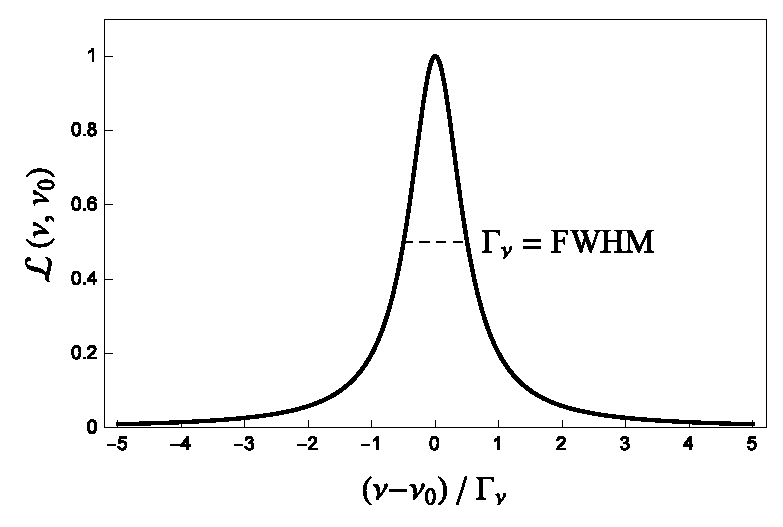
\includegraphics[width=0.6\textwidth]{nLinewidth}
%\caption{The Lorentzian line shape profile for resonance absorption}
%\label{fig:nlinewidth} 
%\end{figure}

\pagebreak
%********************************** % Fifth Section  *************************************
\section{Doppler shifts}  %Section - 1.5

\pagebreak
%********************************** % Sixth Section  *************************************
\section{Behavior of absorption coefficient}  %Section - 1.6

\pagebreak
%********************************** % Seventh Section  *************************************
\section{Non-linear differential equation}  %Section - 1.7

\pagebreak

\section{Relevant data}

\begin{table}[h]
\centering
\begin{tabular*}{0.5\textwidth}{@{\extracolsep{\fill} }l c c}
\toprule
& \multicolumn{2}{c}{Rubidium} \\
\midrule
Isotope & 85 & 87 \\
Atomic mass & 84.911794 & 86.909187 \\
in \(10^{-25}\)kg & 1.40999 & 1.44316 \\
Abundance & 72.17\% & 27.83\% \\
Spin I & \(\sfrac{5}{2}\) & \(\sfrac{3}{2}\) \\
lifetime \(6^{2}P_{3/2}\) & \multicolumn{2}{c}{\SI{112}{\nano\second}} \\
Natural linewidth & \multicolumn{2}{c}{\(2\pi \times \SI{1.421}{\mega\hertz}\) } \\
\bottomrule
\end{tabular*}
\caption{Properties of rubidium isotopes}
\label{table:iso_prop}
\end{table}
\pagebreak

%********************************** % Eighth Section  *************************************

\section{D2 line} %Section - 1.2 

\begin{figure}[h]
\centering
\includegraphics[width=0.9\textwidth]{energylevel}
\caption{\(5^{2}S_{1/2} \rightarrow 6^{2}P_{3/2}\) transition of \(^{85}\)Rb and \(^{87}\)Rb with corresponding hyperfine structure}    
\end{figure}

\vspace{\fill}

The transition of interest is, as we have discussed before, the \(5^{2}S_{1/2} \rightarrow 6^{2}P_{3/2}\) of rubidium. As known rubidium
occurs in two isotopes, \(^{85}\)Rb and \(^{87}\)Rb.
As we can see both isotopes have the same transition energy, but due to the different spin I (see table:~\ref{table:iso_prop}) we get
different energy levels for the groundstate \citep{nist_asd}. This is the reason why we wittness four doppler peaks in our spectrum.
\bigskip

\textbf{Caution:} Both figures below show the correct correlation between energy and isotopes. The reason for this is that the spectrum
shows transition energy and the other one the specific energy levels.

\vspace{\fill}

\begin{figure}[h]
\centering
\includegraphics[width=0.6\textwidth]{spectrum_doppler}
\caption{Doppler spectrum of D2 line}
\label{fig:doppler} 
\end{figure}

\vspace{\fill}

\begin{figure}[h]
\centering
\includegraphics[width=0.6\textwidth]{groundstate}
\caption{Relative energy gaps of the groundstates between both isotopes}
\label{fig:gap} 
\end{figure}